\documentclass{beamer}
\usepackage[utf8]{inputenc}
\usepackage[T1]{fontenc}
\usepackage[polish]{babel}
\usepackage{polski}
\usepackage{indentfirst}
\usepackage{hyperref}
\usepackage{graphicx}
\usepackage{float}
\usepackage{amsmath}
\usepackage{xurl}
\usepackage{tikz}
\usepackage[skip=1ex]{caption}
\usepackage{tabularx}
\usepackage{subfig}
\newcolumntype{C}{>{\centering\arraybackslash}X}
\usepackage{subfiles}
\usepackage{listings}
\usepackage{xparse}
\usepackage{svg}

\AtBeginSection[]{}

\author{Jan Szablanowski}
\title{Zastosowanie algorytmu mrówkowego do CVRP - prezentacja wyników}
\date{07.04.2025}
\usepackage{UCAS}
\usepackage{subfiles}
% defs
\def\cmd#1{\texttt{\color{red}\footnotesize $\backslash$#1}}
\def\env#1{\texttt{\color{blue}\footnotesize #1}}
\definecolor{deepblue}{rgb}{0,0,0.5}
\definecolor{deepred}{rgb}{0.6,0,0}
\definecolor{deepgreen}{rgb}{0,0.5,0}
\definecolor{halfgray}{gray}{0.55}

\def\cmd#1{\texttt{\color{red}\footnotesize $\backslash$#1}}
\def\env#1{\texttt{\color{blue}\footnotesize #1}}
\definecolor{deepblue}{rgb}{0,0,1}
\definecolor{deepred}{rgb}{0.6,0,0}
\definecolor{deepgreen}{rgb}{0,0.5,0}
\definecolor{halfgray}{gray}{0.55}

\lstset{
    basicstyle=\ttfamily\small,
    keywordstyle=\bfseries\color{deepblue},
    emphstyle=\ttfamily\color{deepred},    % Custom highlighting style
    stringstyle=\color{deepgreen},
    numbers=left,
    numberstyle=\small\color{halfgray},
    rulesepcolor=\color{red!20!green!20!blue!20},
    frame=shadowbox,
}
\DeclareDocumentCommand \imgsrc { s O {Image credit} +m }{%
  \IfBooleanTF{#1}{%
        \def\tempa{off}%
        \def\tempb{#3}%
        \ifx\tempa\tempb
          \gdef\@imgsrcnavigation{}%
        \else
          \gdef\@imgsrcnavigation{{\tiny #2:\thinspace #3}}%
        \fi
  }{%
        {\tiny #2:\thinspace #3}%
  }%
}

\begin{document}
\beamertemplatenavigationsymbolsempty
\begin{frame}[plain]
    \begin{figure}
        \begin{center}
            
\includegraphics[width=0.8\linewidth]{img/logo.png}
        \end{center}
    \end{figure}
    \vspace{-4mm}
    \titlepage
\end{frame}

% \begin{frame}
%     \tableofcontents[sectionstyle=show,subsectionstyle=show/shaded/hide,subsubsectionstyle=show/shaded/hide]
% \end{frame}

\section*{Wprowadzenie}

\begin{frame}{Problem CVRP}
    \begin{itemize}
        \setlength\itemsep{1em}
        \item Pojazdy dostarczają towary do klientów z jednego magazynu
        \item Każdy pojazd ma ograniczoną pojemność
        \item Klienci mają różne zapotrzebowanie na towary
        \item Każdy klient musi być odwiedzony dokładnie raz
        \item Celem jest minimalizacja całkowitego kosztu tras
    \end{itemize}
\end{frame}

\begin{frame}{Przykład CVRP}
    \begin{columns}
        \begin{column}{0.55\textwidth}
            \begin{figure}
                \centering
                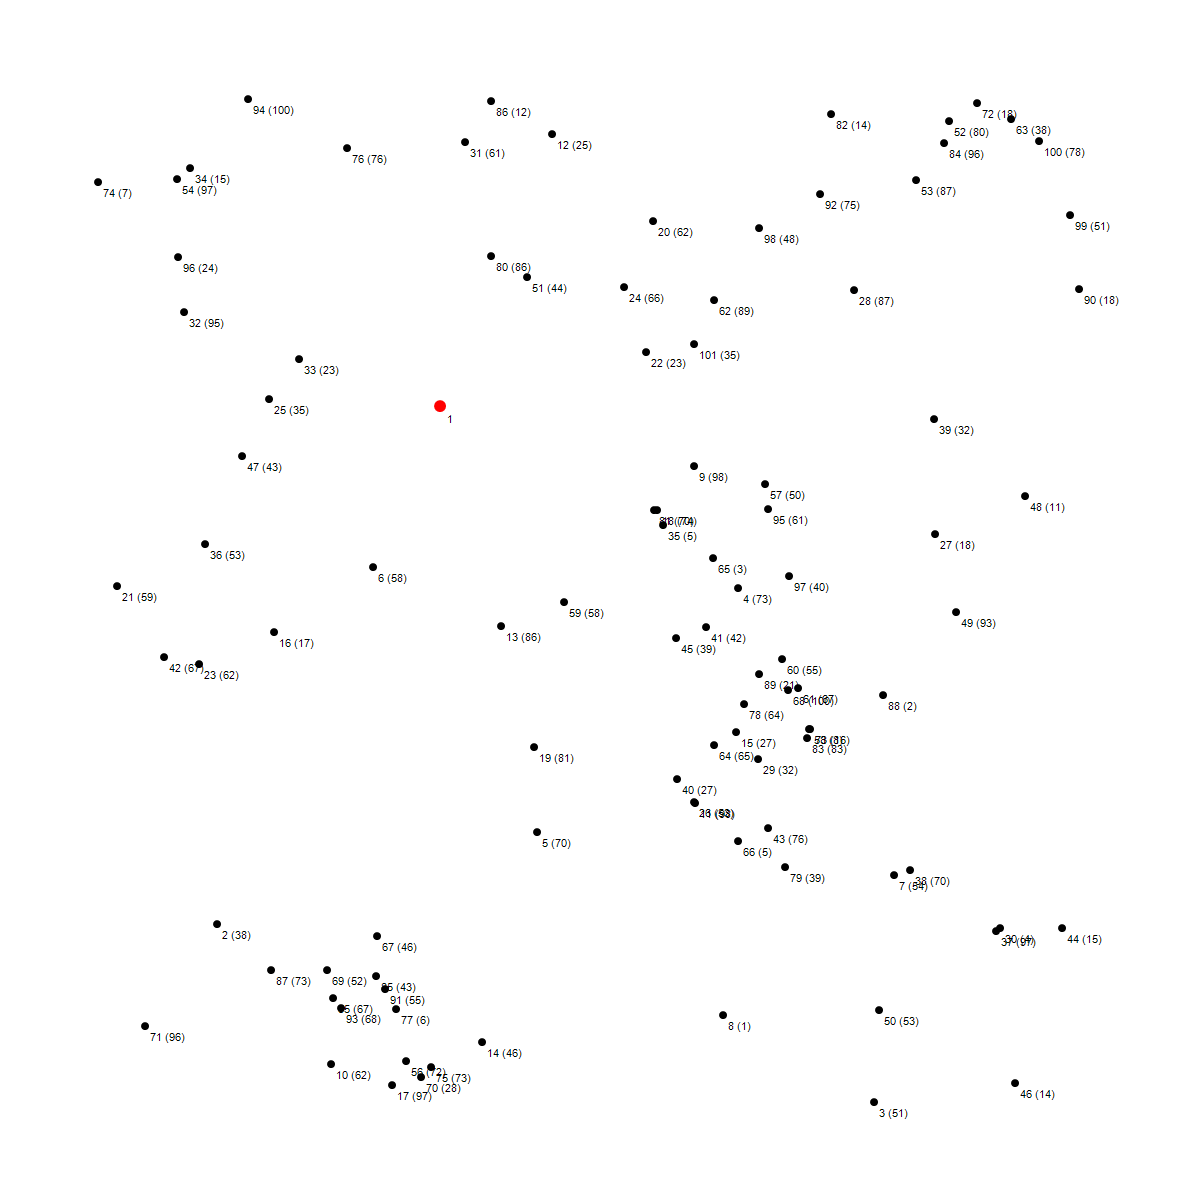
\includegraphics[width=\linewidth]{../report/img/20250405_224145_X-n101-k25.png}
                \caption{Instancja \texttt{X-n101-k25}}
            \end{figure}        
        \end{column}
        \begin{column}{0.55\textwidth}
            \begin{figure}
                \centering
                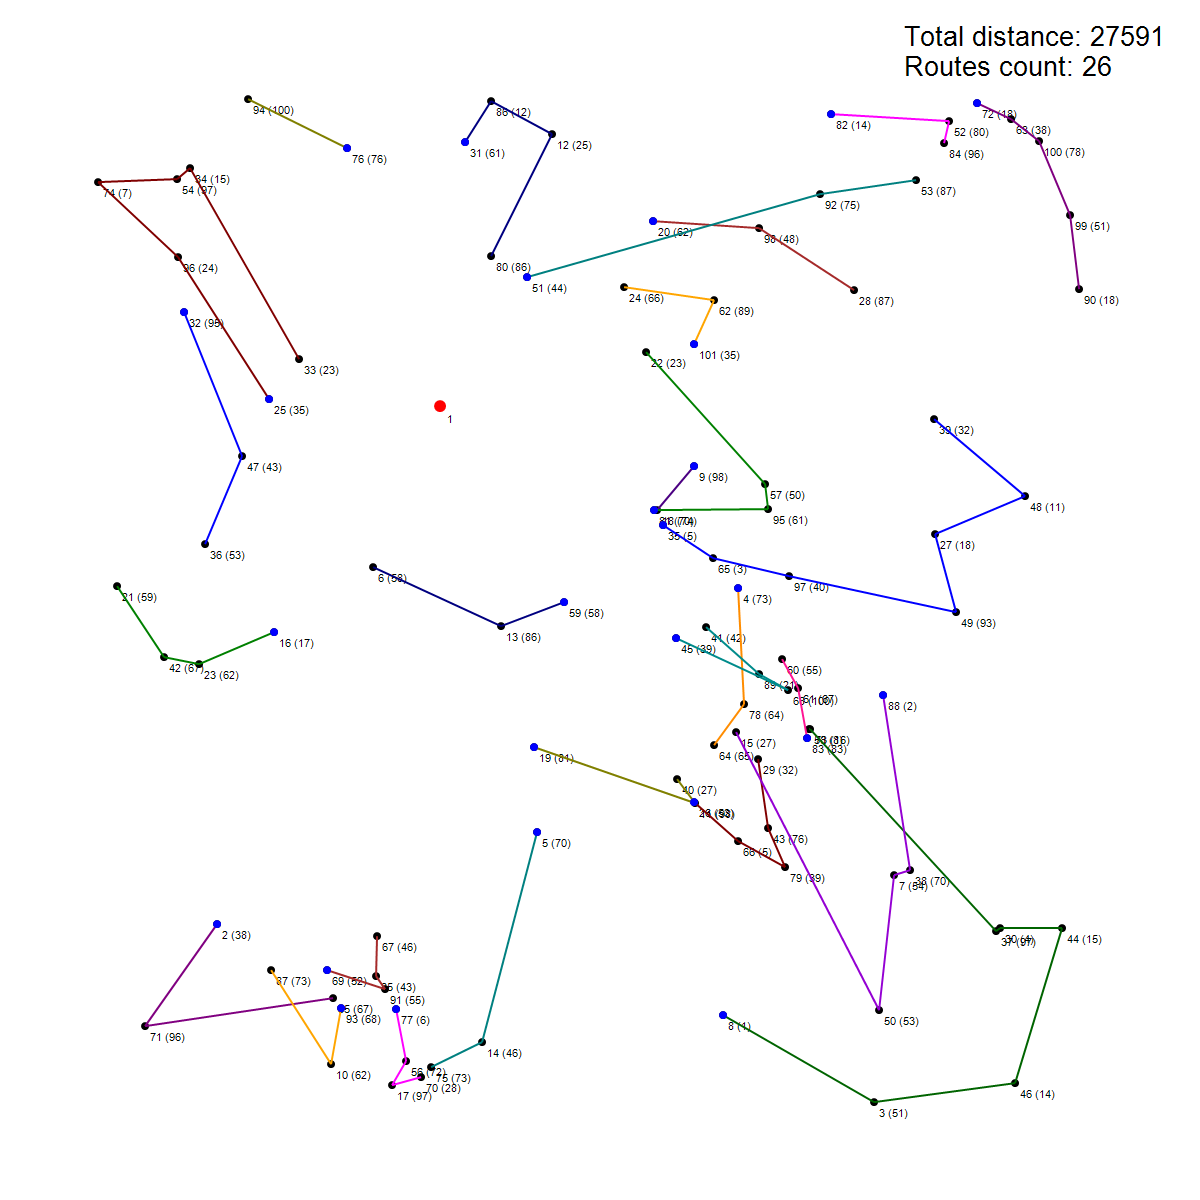
\includegraphics[width=\linewidth]{../report/img/20250407_002013_X-n101-k25_optimal.png}
                \caption{Optymalne rozwiązanie}
            \end{figure}        
        \end{column}
    \end{columns}
\end{frame}

\begin{frame}{Testowane algorytmy}
  \begin{enumerate}
    \setlength\itemsep{1em}
    \item Algorytm mrówkowy (Ant Colony Optimization - ACO) \cite{dorigo}
    \item Algorytm mrówkowy z heurystyką 2-opt \cite{tan}
    \item Algorytm mrówkowy z modyfikacją Max-Min (Max-Min ant system - MMAS) \cite{maxmin}
    \item Algorytm zachłanny (Greedy algorithm)
  \end{enumerate}
\end{frame}

\begin{frame}{Parametry algorytmów ACO i ACO 2-opt}
    % MaxIterations = 100,
    % Alpha = 1.0,
    % Beta = 5.0,
    % EvaporationRate = 0.2,
    % Q = 10,
    % InitialPheromone = 0.1,
    \begin{itemize}
        \setlength\itemsep{1em}
        \item liczba mrówek $=$ liczba wierzchołków
        \item liczba iteracji $= 100$
        \item współczynnik wpływu feromonu $\alpha = 1.0$
        \item współczynnik wpływu heurystyki (odległości) $\beta = 5.0$ 
        \item współczynnik parowania feromonu $EvaporationRate = 0.2$
        \item współczynnik dodawania feromonu $Q = 10$
        \item początkowa ilość feromonu $InitialPheromone = 0.1$
    \end{itemize}
\end{frame}

\begin{frame}{Parametry algorytmu MMAS}
    % PheromoneMin = 0.01,
    % PheromoneMax = pheromoneMax,
    % OnlyBestUpdates = false,
    % StagnationLimit = 20
    \begin{itemize}
        \setlength\itemsep{1em}
        \item minimalna ilość feromonu $PheromoneMin = 0.01$
        \item maksymalna ilość feromonu $PheromoneMax = 10$
        \item początkowa ilość feromonu $InitialPheromone = 10$ 
        \item limit stagnacji (maksymalna liczba iteracji bez poprawy) $StagnationLimit = 20$
    \end{itemize}
\end{frame}

\section*{Hipoteza 1}
\begin{frame}{Hipoteza 1}
    \textit{Algorytm mrówkowy z heurystyką 2-opt znajduje trasy o co najmniej 10\% mniejszym koszcie w porównaniu do klasycznego algorytmu mrówkowego.}
    \vspace{1em}

    \textbf{Wynik: Częściowo potwierdzona dla dużych instancji.} 
\end{frame}

\begin{frame}{Heurystyka 2-opt}
    \begin{itemize}
        \setlength\itemsep{1em}
        \item heurystyka lokalna (ulepsza pojedynczą trasę po jej wyznaczeniu przez kroki algorytmu mrówkowego)
        \item główna idea -- zmiana kolejności odwiedzania klientów w trasie, żeby nie było przecięć tras
        \item heurystyka jest stosowana również w klasycznym TSP
    \end{itemize}
\end{frame}

\begin{frame}{Heurystyka 2-opt -- przykład}
    \begin{figure}
        \centering
        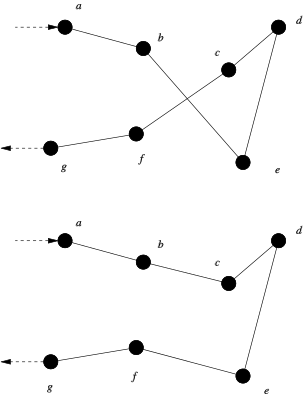
\includegraphics[width=0.5\linewidth]{img/2-opt_wiki.png}
    \end{figure}        
    \imgsrc{PierreSelim, CC BY-SA 3.0, via Wikimedia Commons} 
\end{frame}

\begin{frame}{Wyniki eksperymentów}
    \begin{columns}
        \begin{column}{0.55\textwidth}
            \begin{figure}
                \centering
                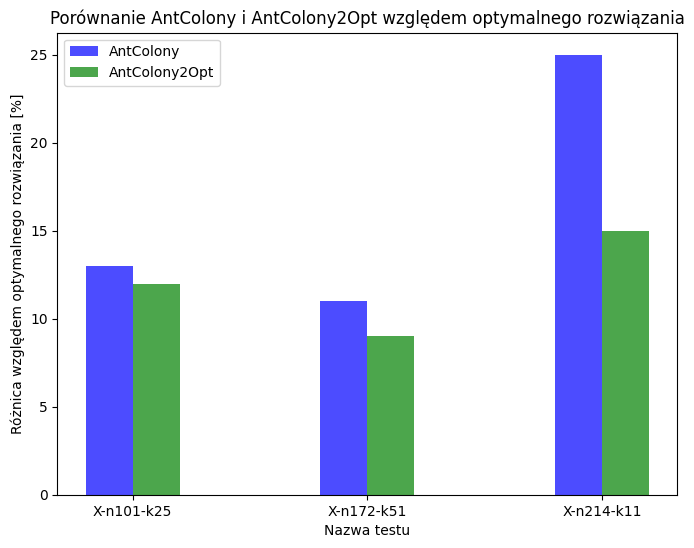
\includegraphics[width=\linewidth]{../report/img/2opt_wzgledem_optymalnego.png}
                \caption{Długość rozwiązania ACO i ACO 2-opt względem optymalnego}
            \end{figure}        
        \end{column}
        \begin{column}{0.55\textwidth}
            \begin{figure}
                \centering
                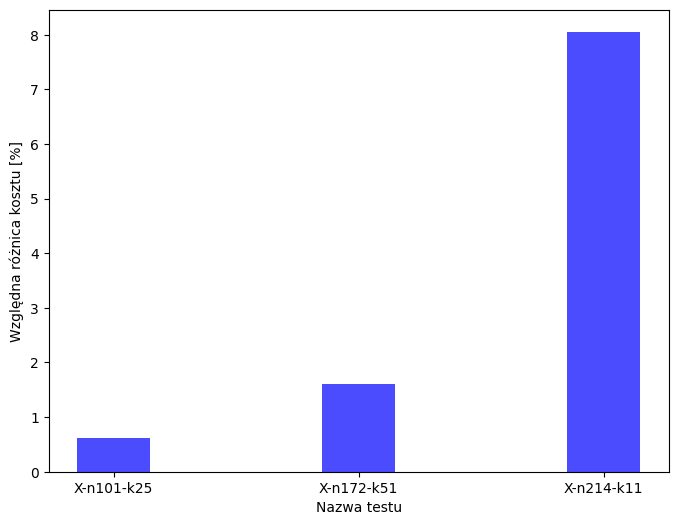
\includegraphics[width=\linewidth]{../report/img/2opt_wzgledem_zwyklego.png}
                \caption{O ile procent AntColony2Opt jest lepszy od AntColony?}
            \end{figure}        
        \end{column}
    \end{columns}
\end{frame}

\section*{Hipoteza 2}

\begin{frame}{Hipoteza 2}
    \textit{Algorytm mrówkowy z modyfikacją Max-Min znajduje rozwiązanie o koszcie nie większym niż 5\% od kosztu rozwiązania znalezionego przez klasyczny algorytm mrówkowy, ale potrzebuje do tego o 10\% mniejszej liczby pojazdów.}
    \vspace{1em}
    
    \textbf{Wynik: Odrzucona.} 
\end{frame}


\begin{frame}{Heurystyka MAX-MIN}
    \begin{itemize}
        \setlength\itemsep{1em}
        \item zmiana sposobu aktualizacji feromonu
        \item feromon na krawędzi jest aktualizowany tylko przez najlepszą mrówkę w danej iteracji lub globalnie
        \item feromon na krawędzi jest ograniczony przez wartości $PheromoneMin$ i $PheromoneMax$
        \item przy braku poprawy przez pewną liczbę iteracji, algorytm resetuje feromon na krawędziach
        \item celem jest zwiększenie jakości rozwiązań (eksploatacja)
    \end{itemize}
\end{frame}


\begin{frame}{Wyniki eksperymentów}
    \begin{columns}
        \begin{column}{0.55\textwidth}
            \begin{figure}
                \centering
                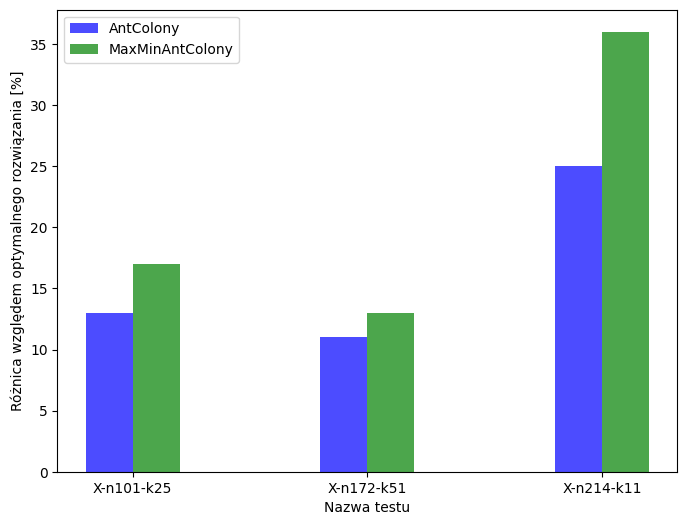
\includegraphics[width=\linewidth]{../report/img/maxmin_wzgledem_optymalnego.png}
                \caption{Długość rozwiązania ACO i MMAS względem optymalnego}
            \end{figure}        
        \end{column}
        \begin{column}{0.55\textwidth}
            \begin{figure}
                \centering
                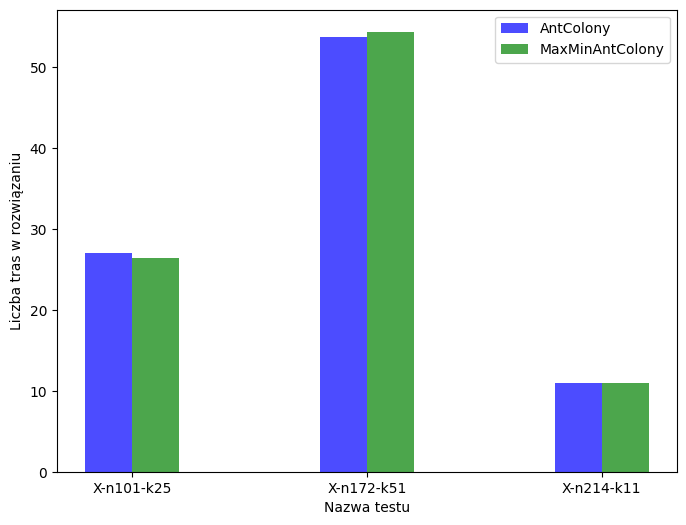
\includegraphics[width=\linewidth]{../report/img/maxmin_trasy.png}
                \caption{Liczba tras dla ACO i MMAS}
            \end{figure}        
        \end{column}
    \end{columns}
\end{frame}

\section*{Hipoteza 3}
\begin{frame}{Hipoteza 3}
    \textit{Procentowa różnica kosztów wyznaczonych tras między algorytmem zachłannym i klasycznym algorytmem mrówkowym rośnie wraz ze wzrostem liczby klientów na niekorzyść algorytmu zachłannego.}
    \vspace{1em}

    \textbf{Wynik: Odrzucona. Potwierdzono hipotezę odwrotną.}
\end{frame}


\begin{frame}{Wyniki eksperymentów}
    \begin{columns}
        \begin{column}{0.55\textwidth}
            \begin{figure}
                \centering
                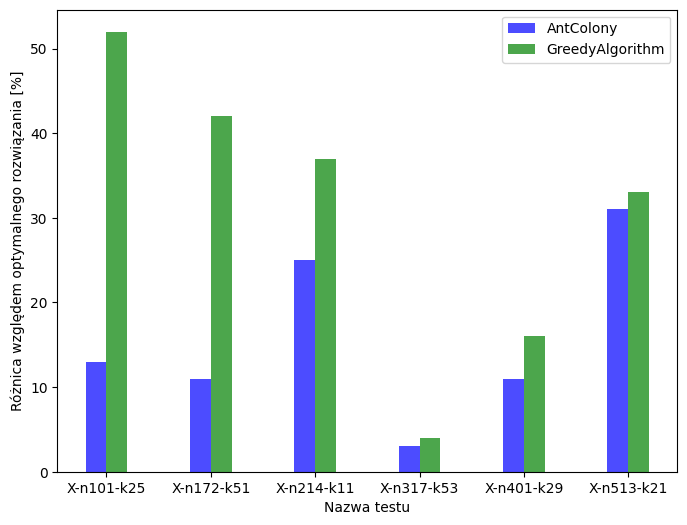
\includegraphics[width=\linewidth]{../report/img/greed_wzgledem_optymalnego.png}
                \caption{Długość rozwiązania ACO i Greedy względem optymalnego}
            \end{figure}        
        \end{column}
        \begin{column}{0.55\textwidth}
            \begin{figure}
                \centering
                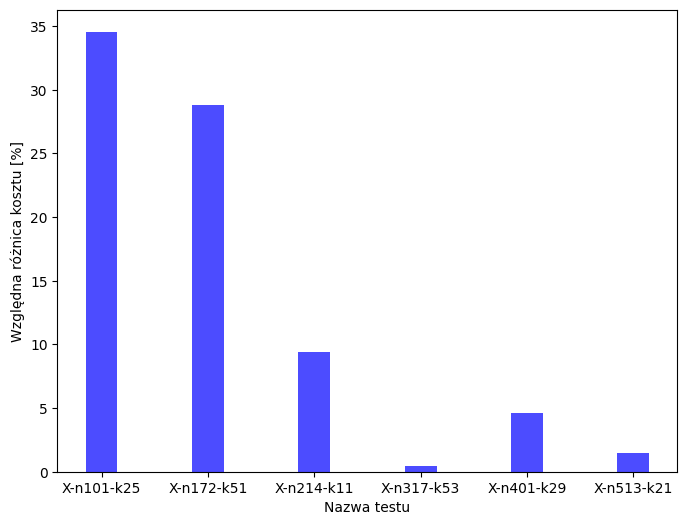
\includegraphics[width=\linewidth]{../report/img/greedy_wzgledem_zwyklego.png}
                \caption{O ile procent ACO jest lepszy od Greedy?}
            \end{figure}        
        \end{column}
    \end{columns}
\end{frame}


\section*{Hipoteza 4}

\begin{frame}{Hipoteza 4}
    \textit{Procentowa różnica kosztów wyznaczonych tras między algorytmem mrówkowym z heurystyką 2-opt i klasycznym algorytmem mrówkowym rośnie wraz ze wzrostem rozproszenia klientów (mierzonego średnią odległością klientów od magazynu) na niekorzyść klasycznego algorytmu.}
    \vspace{1em}

    \textbf{Wynik: Potwierdzona.}
\end{frame}


\begin{frame}{Wyniki eksperymentów}
    \begin{figure}
        \centering
        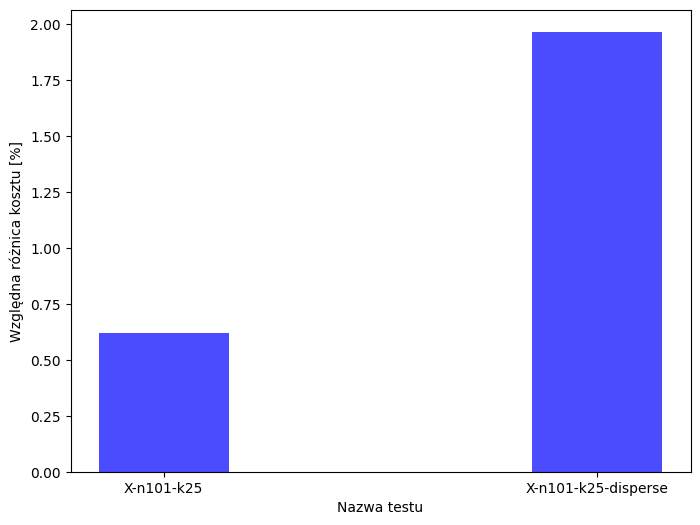
\includegraphics[width=0.7\linewidth]{../report/img/disperse.png}
        \caption{O ile procent AntColony2Opt jest lepszy od AntColony dla różnej wartości rozproszenia klientów?}
    \end{figure}        
\end{frame}

\begin{frame}{Wnioski}
    \begin{itemize}
        \setlength\itemsep{1em}
        \item Algorytm mrówkowy z heurystyką 2-opt osiąga najlepsze wyniki pod względem kosztu rozwiązań
        \item Modyfikacja Max-Min nie przyniosła oczekiwanych korzyści względem klasycznego algorytmu mrówkowego
        \item Różnica między algorytmem zachłannym a mrówkowym zaskakująco maleje wraz ze wzrostem problemu
        \item Zastosowanie heurystyki 2-opt jest szczególnie efektywne dla problemów z dużym rozproszeniem klientów
    \end{itemize}
\end{frame}

\begin{frame}[allowframebreaks]
    \frametitle{Bibliografia}
    \nocite{*}
    \bibliographystyle{unsrt}
    \bibliography{../ref.bib}
\end{frame}

\end{document}